%++++++++++++++++++++++++++++++++++++++++
% Don't modify this section unless you know what you're doing!
\documentclass[letterpaper,12pt]{article}
\usepackage{tabularx} % extra features for tabular environment
\usepackage{amsmath}  % improve math presentation
\usepackage{graphicx} % takes care of graphic including machinery
\usepackage[margin=1in,letterpaper]{geometry} % decreases margins
\usepackage{cite} % takes care of citations
\usepackage[final]{hyperref} % adds hyper links inside the generated pdf file
\hypersetup{
	colorlinks=true,       % false: boxed links; true: colored links
	linkcolor=blue,        % color of internal links
	citecolor=blue,        % color of links to bibliography
	filecolor=magenta,     % color of file links
	urlcolor=blue         
}
%++++++++++++++++++++++++++++++++++++++++


\begin{document}

\title{Pŕactica 1 - VLAN, STP, DHCP y Ruteo Estático}
\author{Matthew Aguerreberry, Natasha Tomattis}
\date{\today}
\maketitle

% \begin{abstract}
% In this experiment we studied a very important physical effect by measuring the
% dependence of a quantity $V$ of the quantity $X$ for two different sample
% temperatures.  Our experimental measurements confirmed the quadratic dependence
% $V = kX^2$ predicted by Someone's first law. The value of the mystery parameter
% $k = 15.4\pm 0.5$~s was extracted from the fit. This value is
% not consistent with the theoretically predicted $k_{theory}=17.34$~s. We attribute this
% discrepancy to low efficiency of our $V$-detector.
% \end{abstract}


\section{VLANs}
\begin{figure}[ht] 
        
        \centering 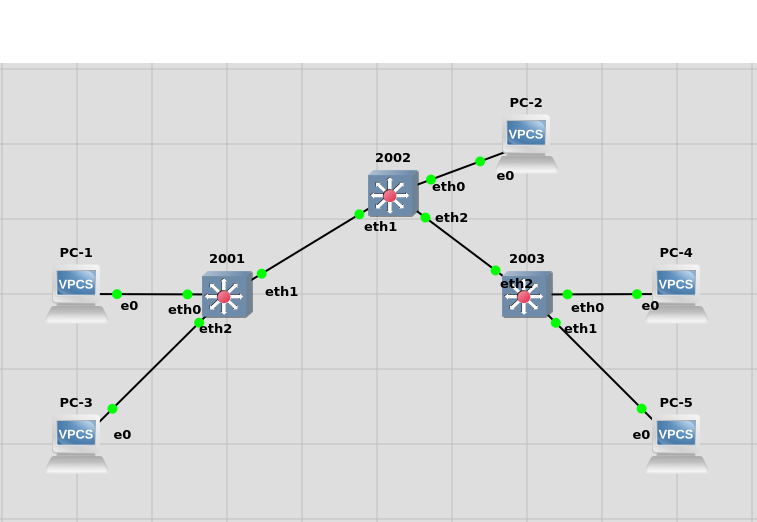
\includegraphics[width=0.8\columnwidth]{lab01.PNG}
        %\includegraphics[width=1.0\columnwidth]{sr_setup.pdf}
        \caption{
                \label{fig:samplesetup} % spaces are big no-no 
                Implementación Ejercicio 1.
        }
\end{figure}
\begin{enumerate}
	\item \textbf{Definir dos VLANs, 10 y 20. Asignar los nodos PC-1, PC-3 y PC5 a la VLAN 10 y los restantes a la VLAN 20. ¿En qué dispositivo se definen las VLANs?}\\
	Se definen las VLAN 10 en los puertos eth0 y eth2 del OvS 2001, VLAN 20 en puerto eth0 OvS 2002, VLAN 20 en eth0 y VLAN 10 en eth1 en OvS 2003.
	\item \textbf{¿Cómo deben definirse los enlaces entre los dispositivos 2001-2002 y 2002-2003 para que sea posible que los nodos de cada VLAN se vean entre ellos? ¿Por que es necesario hacer esto?} \\
	Los enlaces deben definirse en modo troncal(trunk). Esto permite que las interfaces de los dispositivos admitan paquetes de diferentes VLANs en un mismo enlace.
	\item \textbf{¿Que nombre reciben los puertos donde se conectan las PCs? ¿Es necesario realizar alguna configuración especial en las PCs para que funcionen en un VLAN en particular?}\\
	Los puertos donde se conectan las PC reciben el nombre de puertos de acceso. No es necesario configurar algo especial en las PCs, para ellas las VLAN son transparentes.
	\item \textbf{Realizar las configuraciones correspondientes en todos los switchs para lograr esa conectividad.}\\
	En el switch \textbf{2001} se configuran los puertos eth0 y eth2 como de acceso a la VLAN 10 y el puerto eth1 como trunk (permite el paso de VLAN 10). En el switch \textbf{2002} se configura el puerto eth0 como de acceso a la VLAN 20 y los puertos eth1 y eth2 como trunk(eth1 permite el paso de VLAN 10 y eth2 permite el paso de VLAN 10 y 20). En el switch \textbf{2003} se configura el puerto eth0 como de acceso a la VLAN 20, el puerto eth1 como de acceso a la VLAN 10 y el puerto eth2 como trunk.
	\item \textbf{Utilizar la red 192.168.10.0/26 para la VLAN 10 y la 192.168.10.128/26 para la VLAN 20 y asignar una IP a cada uno de los nodos.} \\
	\item \textbf{Comprobar que los nodos de cada VLAN se pueden comunicar entre ellos, pero no con los nodos de la otra VLAN.} \\
	\item \textbf{¿Que modificación sufre una trama Ethernet para poder adecuarse al trunking de VLANs?.} \\
	Se le agrega una etiqueta extra con los campos definidos en IEEE 802.1q.
	\item \textbf{¿Cual es el número máximo de VLANs que se pueden definir? ¿A qué se debe este máximo?.} \\
	El tamaño del campo VLAN ID es de 12 bits por ende el número máximo es 4096. 
	\item \textbf{Capturar tráfico entre los dispositivos 2001 y 2002 y hacer un ping entre los nodos de la misma VLAN. ¿Qué información es transportada en la trama?.} \\
	Dentro de la trama ethernet está encapsulado los campos 802.1q y aquí se encuentra el VLAN ID. \\
	\item \textbf{¿Que debería utilizar si desea conectar ambas VLANs?.} \\
	Un router \textit{one armed router} o \textit{on a stick}, o un switch capa 3.\\
	\item \textbf{Investigar QinQ (IEEE Standard 802.1.ad).} \\
	Permite insertar múltiples etiquetas VLAN en una misma trama ethernet; juntas crean una jerarquía de etiquetas siendo la etiqueta más cerca del payload la última en ser leída.
\end{enumerate}
\subsection{Enlaces consultados}
\begin{itemize}
    \item{VLAN Trunking to Guest Domains with Open vSwitch} \emph{VLAN Trunking to Guest Domains with Open vSwitch},  available at \url{https://blog.scottlowe.org/2013/05/28/vlan-trunking-to-guest-domains-with-open-vswitch/}.
    
    \item{VLAN Configuration on Open vswitch} \emph{VLAN Configuration on Open vswitch},  available at \url{https://medium.com/@arrosid/vlan-configuration-on-open-vswitch-83459d8c0cfc}.
    
    \item{VLAN TRUNKING CONFIGURATION ON OPEN VSWITCH} available at \url{https://medium.com/@arrosid/vlan-trunking-configuration-on-open-vswitch-f598a965c28}.
\end{itemize}
\section{VLAN, DHCP y Ruteo Estático}
\begin{figure}[ht] 
        
        \centering 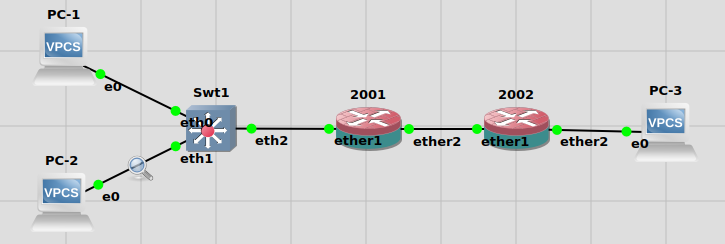
\includegraphics[width=0.8\columnwidth]{lab12topo.PNG}
        %\includegraphics[width=1.0\columnwidth]{sr_setup.pdf}
        \caption{
                \label{fig:samplesetup} % spaces are big no-no 
                Implementación Ejercicio 2.
        }
\end{figure}
\begin{enumerate}
    \item \textbf{¿Es necesario definir alguno de los enlaces como trunk? ¿Cuál?} \\
    Si, el enlace entre \textit{Swt1} y el router \textit{2001} debe ser configurado como trunk.
    
    \item \textbf{Cada PC de la VLAN debe obtener dinámicamente su dirección IP. ¿Qué significan las letras DORA?} \\
    El proceso de DHCP consiste de 4 etapas. Estas etapas se resumen como DORA, Discover, Offer, Rquest y Acknowledgement. 

    \item \textbf{Realizar una captura para ver el funcionamiento del protocolo DHCP. ¿Qué direcciones IP son utilizadas en cada uno de los mensajes?}
    \begin{figure}[ht] 
        
        \centering 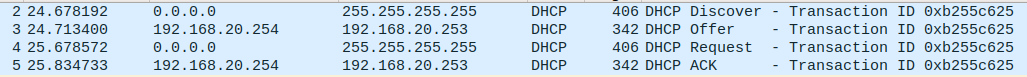
\includegraphics[width=0.8\columnwidth]{lab12.PNG}
        %\includegraphics[width=1.0\columnwidth]{sr_setup.pdf}
        \caption{
                \label{fig:samplesetup} 
                Captura mensajes DORA.
        }
    \end{figure}

    \item \textbf{¿Se pueden conectar las PCs entre las diferentes VLANs? ¿Por qué?} \\
    Si, el router 2001 tiene directamente conectadas ambas VLAN por ende puede rutear el tráfico entre ellas. 
    
    \item \textbf{¿Es posible que el servidor de DHCP se encuentre en el router 2002? Si es así, modifique la configuración para lograr esto.?} \\
    Sí, se configura el router 2001 como DHCP Relay y en el router 2002 se configuran los pool de direcciones y el DHCP Server.
    
    \item \textbf{¿Cómo reconoce el servidor DHCP en 2002 de cuál pool de conexiones tiene que retornar una dirección IP cuando le llegue una solicitud por la interface ether1? Realizar una captura entre los routers 2001 y 2002 para ver esta información.} \\
    
    Cuando se configura el servidor DHCP en 2002 uno debe indicar que direcciones relay se van a aceptar y asignarles un pool de direcciones a cada relay. Como se puede ver en la imagen, cuando llega un mensaje de discover trae consigo la direccion IP de relay, luego el server puede identificar que pool usar.
    
    \begin{figure}[ht] 
        \centering 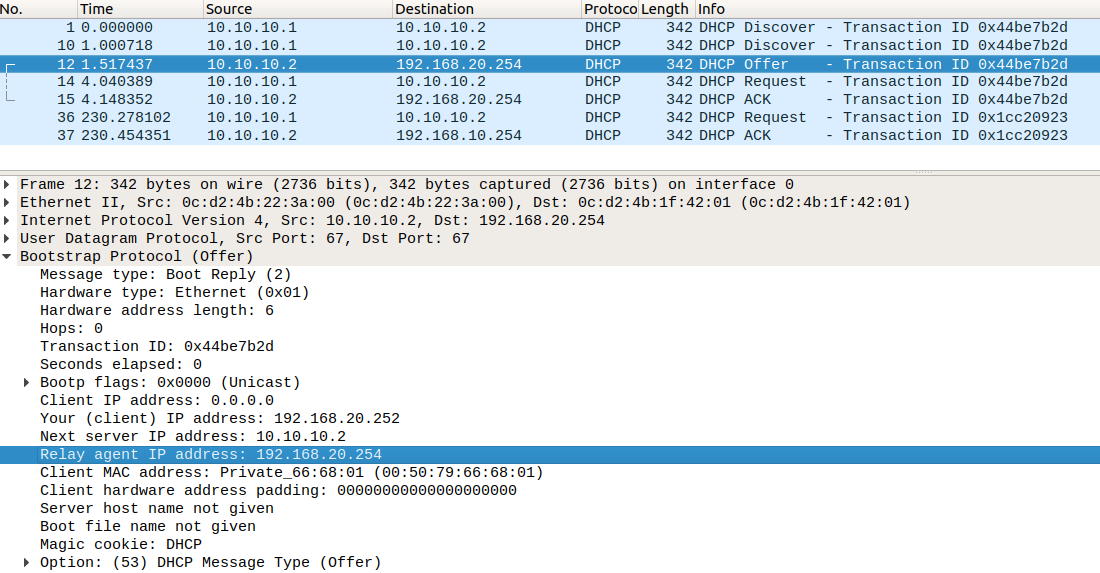
\includegraphics[width=0.8\columnwidth]{lab12relay.PNG}
        %\includegraphics[width=1.0\columnwidth]{sr_setup.pdf}
        \caption{
                \label{fig:samplesetup} 
                Captura entre router 2001 y 2002.
        }
    \end{figure}
    
    \item \textbf{¿Recomienda usar DHCP para asignar IP a un servidor, impresora o un router? ¿Por qué? ¿Es posible lograr que DHCP siempre le asigne la misma IP a un dispositivo?.} \\
    No, ya que son dispositivos que deben mantener una IP estática porque hay servicios que dependen de esta IP. Se puede configurar una asignación estática de IP en el servidor DHCP reconociendo al cliente por el campo \textit{Client MAC Address} del paquete DHCP Discover. En Mikrotik esto se configura desde el menu \textit{/ip dhcp-server lease} con el comando \textit{make-static}.    
\end{enumerate}

\subsection{Enlaces consultados}
\begin{itemize}
    \item{Mikrotik Docs: Manual:IP/DHCP Server} \emph{Mikrotik Docs: Manual:IP/DHCP Server},  available at \url{https://wiki.mikrotik.com/wiki/Manual:IP/DHCP_Server}.
    \item{Mikrotik Docs: Manual:IP/DHCP Relay} \emph{Mikrotik Docs: Manual:IP/DHCP Relay},  available at \url{https://wiki.mikrotik.com/wiki/Manual:IP/DHCP_Relay}.
\end{itemize}
\end{document}
